
% this file is called up by thesis.tex
% content in this file will be fed into the main document

\chapter{Przebieg integracji} % top level followed by section, subsection


% ----------------------- paths to graphics ------------------------

% change according to folder and file names
\ifpdf
    \graphicspath{{8/figures/PNG/}{8/figures/PDF/}{8/figures/}}
\else
    \graphicspath{{8/figures/EPS/}{8/figures/}}
\fi

% ----------------------- contents from here ------------------------

Rozdział ten przedstawia konkretną konfigurację systemu SpeechProcessingPlatform, która została użyta do przeprowadzenia testów opisanych w kolejnym rozdziale, a także opisuje krok po kroku proces integracji usług w systemie SpeechProcessingPlatform na przykładzie usługi IVONA SaaS.
\section{Przykładowa konfiguracja}

\begin{figure}[!h]
	\centering
	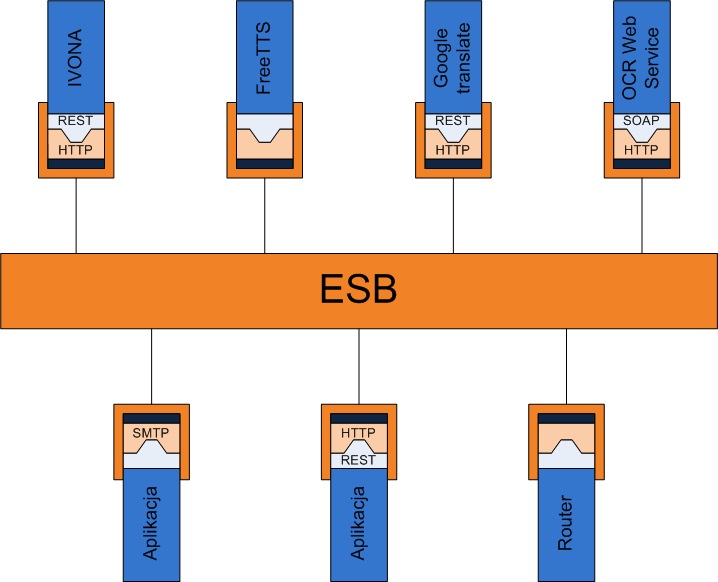
\includegraphics[scale=0.6]{esb.png}
	\caption{Przykładowa konfiguracja  systemu SpeechProcessingPlatform}\label{fig:esb_configuration}
\end{figure}

Rysunek \ref{fig:esb_configuration} przedstawia przykładową konfigurację platformy, która została wykorzystana do przeprowadzenia testów oraz weryfikacji proponowanej architektury. W tym celu z systemem zostały zintegrowane następujące usługi:

\begin{itemize}
	\item TTS
	\begin{itemize}
		\item IVONA SaaS
		\item FreeTTS
	\end{itemize}
	\item Translacja
	\begin{itemize}
		\item Google Translate
	\end{itemize}
	\item OCR
	\begin{itemize}
		\item OCR Web Service
	\end{itemize}
\end{itemize}

\section {Przebieg integracji}

Proces integracji jest unikalny dla każdej usługi. Zależy on od wielu czynników takich jak:

\begin{itemize}
	\item protokół komunikacji
	\item oczekiwany format danych
	\item nazewnictwo metod i parametrów
	\item sekwencja komunikacji
\end{itemize}

Mimo tego można przedstawić proces integracji w postaci kroków, które należy podjąć aby usługa była w pełni zintegrowana z systemem. Kroki te zostaną przedstawione na przykładzie usługi IVONA SaaS.

\subsection {Krok nr 1: Przygotowania}
Krok ten obejmuje wszelkie działania niezwiązane z implementacją, lecz wymagane aby integracja w pełni się powiodła np. rejestracja w usłudze czy instalacja odpowiednich bibliotek.

Ponieważ IVONA SaaS jest usługą płatną, pierwszą rzeczą, którą należy wykonać jest założenie konta na stronie usługi. Informacje podane podczas rejestracji będą potrzebne przy każdorazowej komunikacji z usługą w celu autoryzacji. W prezentowanej konfiguracji do integracji usługi IVONA użyto technologi REST, ale możliwe jest również użycie innych technologii. Po stronie systemu, do integracji użyto technologii JAX-RS, która ułatwia dostęp do usług zgodnych z wybraną do tej integracji technologią. Apache ServiceMix jest dystrybuowany z dużą ilością technologii integracyjnych dzięki czemu większość używanych bibliotek nie musi być dodana bezpośrednio do budowanej aplikacji. Aby było możliwe używanie danej technologii, wystarczy poszukać odpowiedniego zbioru paczek (\textit{feature}) i zainstalować go w kontenerze OSGi, co sprowadza się do wywołania odpowiedniej komendy z konsoli kontenera. W przypadku JAX-RS komenda ta ma postać następującą: 
\begin{center}
features:install cxf-jaxrs
\end{center}

\subsection {Krok nr 2: Implementacja komunikacji}

W kroku tym należy zaimplementować komunikację między systemem a usługą zgodnie z wybraną technologią i wymaganiami narzucanymi przez usługę. Ten etap będzie najbardziej zróżnicowany pomiędzy różnymi usługami.

W przypadku usługi IVONA komunikacja sprowadza się do wykonania żądania HTTP POST pod odpowiedni adres: http://www.ivona.com/api/saas/rest/speechfiles/. Jednak aby komunikacja powiodła się należy poddać się autoryzacji. Usługa IVONA używa autoryzacji opartej o tokeny. Każdy token może być użyty tylko raz i jest ważny przez pięć minut, dlatego każdą operację należy poprzedzić wygenerowaniem nowego tokenu. Po otrzymaniu tokenu należy wygenerować skrót md5 z kombinacji tokenu i hasła podanego podczas rejestracji, który razem z tokenem musi zostać przesłany jako jeden z parametrów wywoływanej operacji. Fragment kodu \ref{lst:ivona_token} przedstawia proces generowania tokenu.

\lstset{language=Java, tabsize=4, caption=Proces generowania tokenu usługi IVONA,label=lst:ivona_token}

\begin{center}
\begin{lstlisting}
public class IvonaTextToSpeechService implements MessageEnabledService, TTSService {
	...
	//metoda zwracajaca gotowy do wywolania obiekt WebClient
	private WebClient getClient() {
		WebClient client = WebClient.create("http://www.ivona.com");
		client.path("/api/saas/rest/");
		client.type("application/x-www-form-urlencoded");
		return client;
	}

	//metoda generujaca token do autoryzacji
	private String getToken() {
		WebClient client = getClient();
		client.path("tokens");
		MultivaluedMap<String, String> tokenParams = new MetadataMap<String, String>();
		tokenParams.putSingle("email", EMAIL);
		String token = client.post(tokenParams,String.class);
		token = token.substring(1, token.length() -1);
		return token;
	}

	//metoda generujaca skrot md5 z godnie z wymagana formula
	private String generateMD5(token) {
		String md5 = createMD5FromString(PASSWORD);
		md5 += token;
		md5 = createMD5FromString(md5);
		return md5;
	}
	...
}
\end{lstlisting}
\end{center} 

Po wygenerowaniu tokenu można przejść do właściwej operacji czyli do generowania dźwięku. Aby tego dokonać należy przygotować obiekt zawierający wszystkie parametry dotyczące procesu generacji w postaci klucz-wartość i wysłać go razem z żądaniem wygenerowania dźwięku. Ponieważ każda usługa posiada swoje własne nazewnictwo parametrów, trzeba dokonać odpowiedniego mapowania. 
Odpowiedź usługi na żądanie przetwarzania jest w formacie JSON i zawiera ona adres URL pliku dźwiękowego. Plik ten należy pobrać i zapisać w postaci binarnej w obiekcie wiadomości jako dane wyjściowe tego etapu przetwarzania. Fragment kodu \ref{lst:ivona_speech} przedstawia proces generowania mowy oraz obsługę otrzymanej odpowiedzi.

\lstset{language=Java, tabsize=4, caption=Proces generowania tokenu usługi IVONA,label=lst:ivona_speech}

\begin{center}
\begin{lstlisting}
public class IvonaTextToSpeechService implements MessageEnabledService, TTSService {
	...
	public Task processTask(Task task) {
		String token = getToken();

		MultivaluedMap<String, String> voiceParams = new MetadataMap<String, String>();
		voiceParams.putSingle("token", token);
		voiceParams.putSingle("md5",generateMD5(token));
		voiceParams.putSingle("text", getTextFromTask(task));
		//mapowanie parametrow przetwarazania dla uslugi IVONA
		setProcessingParams(voiceParams, task)

		WebClient client = getClient();
		client.path("speechfiles");
	
		Response response = client.post(getVoiceParams);
		String soundUrl = getSoundUrlFromResponse(response);
		task.setOuputData(getSoundData(soundUrl);

		return task;
	}
	...
}
\end{lstlisting}
\end{center} 

\subsection {Krok nr 3: Implementacja obsługi wiadomości}

W kroku tym należy dodać obsługę wiadomości do komponentu odpowiadającego za komunikację. Proces ten może okazać się niepotrzebny, jeżeli technologia użyta w kroku nr. 2 dodaje wymaganą funkcjonalność.

W przypadku usługi IVONA, funkcjonalność tą otrzymano przy pomocy nowej ścieżki Apache Camel, której elementem centralnym będzie opisana wcześniej klasa. Fragment \ref{lst:camel_ivona} przedstawia definicję ścieżki Apache Camel dla komponentu IvonaTe	xtToSpeechService.

\lstset{language=XML, tabsize=4, caption=Ścieżka Apache Camel dla komponentu IvonaTextToSpeechService.,label=lst:camel_ivona}

\begin{center}
\begin{lstlisting}
<bean id="ivonaTextToSpeechService" class="pl.edu.agh.speechprocessing.services.IvonaTextToSpeechService"/>

<camelContext xmlns="http://camel.apache.org/schema/spring">

	<route>
		<from uri="nmr:IvonaTextToSpeechService"/>
		<bean ref="ivonaTextToSpeechService" method="process"/>
		<dynamicRouter>
			<method ref="ivonaTextToSpeechService" method="getReturnAddress" />
		</dynamicRouter>
	</route>

</camelContext>
\end{lstlisting}
\end{center}

\subsection {Krok nr 4: Rejestracja komponentu}

Ostatnim krokiem wymaganym aby usługa była w pełni zintegrowana w platformie jest rejestracja komponentu w rejestrze OSGi co umożliwi jego wyszukanie podczas procesu routowania. Proces ten będzie w większości identyczny niezależnie od integrowanej usługi.
W celu poprawnej rejestracji, klasa IvonaTextToSpeechService implementuje dwa interfejsy TTSService oraz MessageEnabledService. Pierwszy z nich służy tylko do oznaczenia typu przetwarzania jaki oferuje dany komponent a drugi wymusza implementację metody zwracającej adres pod którym komponent będzie nasłuchiwał na przychodzące wiadomości. Dodatkowo, podczas rejestracji należy podać parametry przetwarzania, które są obsługiwane przez daną usługę.

\lstset{language=Java, tabsize=4, caption=Implementacja metody z interfejsu MessageEnabledService. ,label=lst:ivona_message}

\begin{minipage}{\linewidth}
\begin{center}
\begin{lstlisting}
public class IvonaTextToSpeechService implements MessageEnabledService, TTSService {
	...
	public String getServiceURI() {
		return "nmr:IvonaTextToSpeechService";
	}

	...
}
\end{lstlisting}
\end{center} 
\end{minipage}

\lstset{language=XML, tabsize=4, caption=Rejestracja komponentu IvonaTextToSpeechService w rejestrze OSGi przy użyciu kontenera Blueprint.,label=lst:ivona_blueprint_definition}

%SPRAWDZIĆ
\begin{center}
\begin{lstlisting}
<blueprint xmlns="http://www.osgi.org/xmlns/blueprint/v1.0.0">
	<bean id="ivonaTextToSpeechService" class="pl.edu.agh.speechprocessing.services.IvonaTextToSpeechService"/>
	<service ref="ivonaTextToSpeechService" auto-export="interfaces" ranking="8">
		<service-properties>
			<entry key="language">
				<set value-type="java.lang.String">
					<value>en</value>
					<value>it</value>
					<value>pl</value>
					<value>de</value>
				</set> 
			</entry>
			<entry key="audioFormat">
				<set value-type="java.lang.String">
					<value>mp3</value>
					<value>ogg</value>
					<value>pcm16</value>
				</set> 
			</entry>
		</service-properties>
	</service>
</blueprint>

\end{lstlisting}
\end{center}

\section*{Podsumowanie} 
Powyższy rozdział przedstawił proces integracji usług w platformie SpeechProcessingPlatform. Jak widać proces ten nie jest zbyt skomplikowany i można go zastosować do integracji dowolnej usługi. Oczywiście będzie on wymagał pewnych modyfikacji, których główny powodem są różnice w obsługiwanych protokołach komunikacji.

 

% ---------------------------------------------------------------------------
%: ----------------------- end of thesis sub-document ------------------------
% ---------------------------------------------------------------------------



 






